\section{Plato: A model-aware DBMS}
\label{sec:architecture}

\begin{figure}
\center
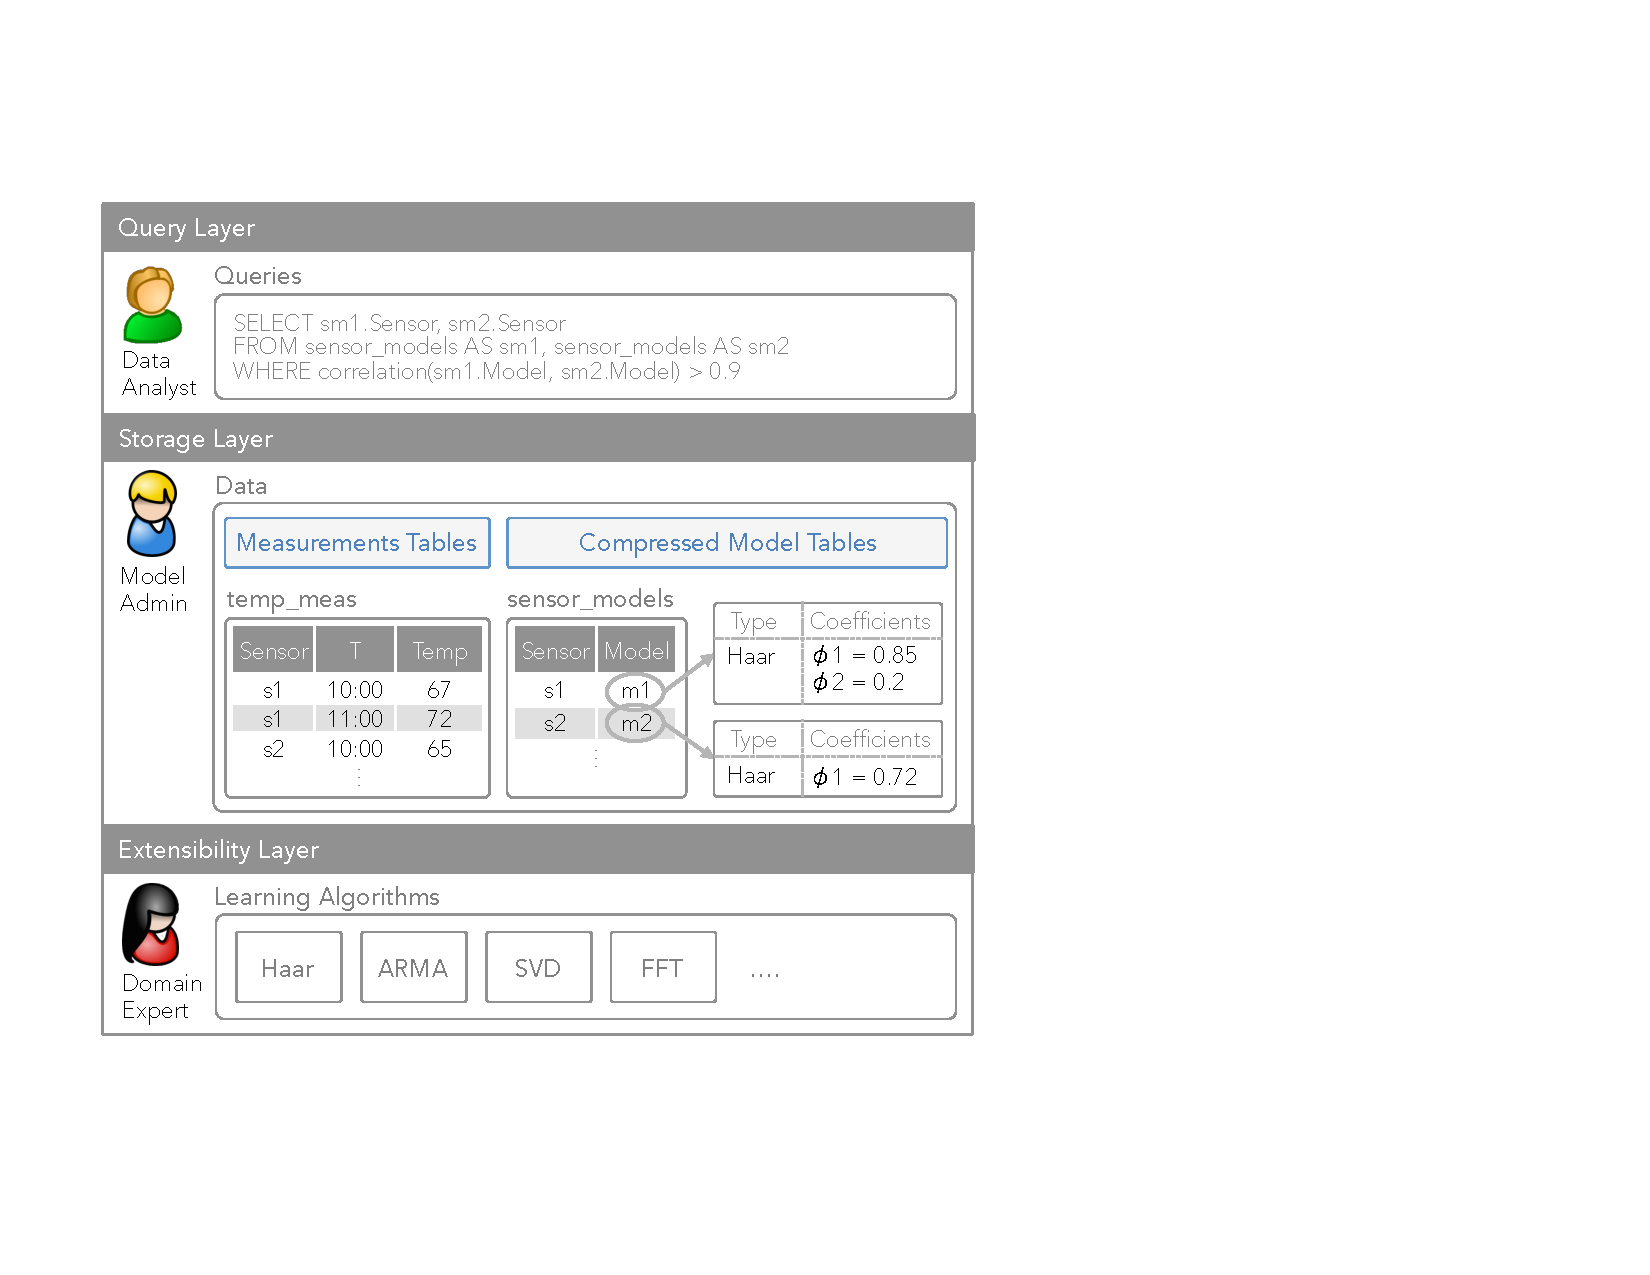
\includegraphics[width=\columnwidth]{fig-architecture2.pdf}
\caption{\projName's Architecture}
\label{fig:basic-architecture}
\vspace{-0.4cm}
\end{figure}

\projName\ enables declarative and efficient querying of spatiotemporal sensor data through the architecture shown in Figure~\ref{fig:basic-architecture}. The system interacts with three different types of users: \emph{Domain experts} with knowledge of statistics and signal processing write learning algorithms, which given raw data create a model over the data using a particular statistical technique (e.g., Wavelets, Fast Fourier Transform, etc).
Out of these registered learning algorithms, \emph{model administrators} with knowledge of a particular dataset, choose a learning algorithm and instantiate its parameters to create a good model for the particular data set. Finally, \emph{data analysts} query the generated models using a declarative query language. We next present the components of \projName\ enabling this workflow. As our running example, we will be using temperature data collected from sensors placed in offices across UC San Diego's campus, in the context of the Energy Dashboard project\footnote{http://energy.ucsd.edu}.

\subsection{Preliminaries}
\label{sec:prelims}

A Plato database consists of {\em measurements}, {\em samples} and {\em models}.


\noindent {\bf A Measurement Table} In the interest of
simplicity let us first assume that the database has a single table
$T$ with measurements. The table $T$ has {\em dimension attributes}
and {\em measurement attributes}. The dimension attributes define the
time and place where the measurement was taken.

In the case of spatiotemporal sensor data, we further classify the
dimension attributes into {\em metadata} attributes and {\em
  spatiotemporal} attributes. We also assume that the domain of each
measurement attribute is the set of reals $R$.

%In another example, consider a table \texttt{Air1(Sensor, T, co, no2)}.

\noindent{\bf Sample table:} From the raw measurement tables the model
admin creates the sample. The goal of the mapping from the measurement
table to the sample table is to create rows that correspond to
independent draws from a distribution.

Doing so might require pivoting, difference taking and other manipulation.

We now review the central concepts of probability theory. In the next
paragraph we will link these concepts back to the example above.
Formally, a probability space is defined as a triplet: $\langle
\Omega, \sigma, P  \rangle$. We now elaborate on these three elements.
\begin{itemize}
\item {\bf $\Omega$} The sample space is the set of all possible outcomes.
\item {\bf $\sigma$} A set of subsets of
  $\Omega$. By convension, these subsets are called {\em events}.~\footnote{Technically, if $\Omega$ is uncountably
  infinite, one cannot define $P$ for {\em all} subsets of
  $\Omega$. Instead, $P$ is defined over a collection of subsets that
  are ``Measurable''. A full description of measurability and it's
  relation to probability is beyond the scope of this paper.}
\item {\bf $P$} The probability is a function from elements of
  $\sigma$ (i.e. subsets of $\Omega$) to the segment $[0,1]$. The function $P$
  has to obey the three axioms of probability:
\begin{itemize}
\item If $E \subseteq \Omega$, $P(E) \geq 0$.  
\item $P(\Omega)=1$.
\item If $E_1,E_2,E_3,... \subseteq \Omega$ are disjoint sets. Then 
$$ P\left(\bigcup_{i=1}^{\infty} E_i \right)=\sum_{i=1}^{\infty}
  P(E_i) $$
\end{itemize}
\end{itemize}

One more concept, {\em random variables}, is needed in order to
connect probability distributions back to tables. A random variable is
a mapping from $\Omega$ to the real numbers (which can be restricted
to a smaller set, such as the integers). The random variable $X$ connects
the abstract outcome $\omega \in \Omega$ with the value of a
particular attribute $X(\omega)$.
\yannisp{The probability theory presented up to this point should be considered already known. YK will eventually condense that part to essentially a listing of the relevant terms. E.g., I assume the relevant ICDT reader is already aware of the axioms of a probability function.} 
$(\mbox{Sensor}(\omega),X(\omega),Y(\omega),Z(\omega),T(\omega),\mbox{co}(\omega),\mbox{no2}(\omega))$.

For example, consider a table \texttt{Air2(Sensor, X, Y, T, co,
  no2)}. The \texttt{Sensor} is a metadata attribute that provides the
id of a sensor as a natural number (we deonte the set of all natural
numbers $N$. The spatiotemporal attributes \texttt{X}, \texttt{Y}
and \texttt{T} provide the time and place of the sensor
measurements. The measurement attributes \texttt{co} and \texttt{no2}
provide the values of CO and NO2 measured by the sensor. These five
attributes are specified by real numbers (we denote the real numbers
by $R$).

Note that the example allows the sensors to be mobile, hence the
same sensor may report measurements from different locations. For the
rest of this paper we will use $X$, $Y$, $Z$, and $T$ to denote the 
the relational attributes corresponding to the three spatial
components and the temporal component, respectively.


{\em Models} are approximations of the underlying distribution $P$.

\yoav{I am not sure where to continue from here. I can see many
  options, but we should probably talk.}

Let us call ${\cal D_T}$ the domain of the dimensions of the table
$T$. In the running example, assuming ${\cal D}_{xyt}$ is the
spatiotemporal domain that includes the 2D space and time and ${\cal
  S}$ is the domain of sensor id's (eg, the integers), then the users
may assume that ${\cal D} = {\cal S} \times {\cal
  D}_{xyt}$. Alternately, the users may assume that ${\cal D}_{desc}$
describes the dimensions included in the relevant subspace together
with any range restrictions. For instance, ${\cal D}_{xy:
  (x-x_0)^2+(y-y_0)^2 = r^2}$ contains all 2D points within a circle
centered at $(x_0, y_0)$ with radius $r$. \\

\[ 
\begin{array}{l}
F(d_1, \ldots, d_k, m_1, \ldots, m_l) = \\
P(M_1 \leq m_1, \ldots, M_l \leq m_l | D_1 = d_1, \ldots, D_k = d_k) \\
\end{array}
\]

Given values $d_1,\ldots,d_k$ for the $k$ dimension attributes, a tuple $t=(d_1,\ldots,d_k,m_1,\ldots,m_l)$ of the measurements table $T$ (i.e., the measurement values $m_1, \ldots, m_l$) is a sample drawn from the probability distribution. \yannisp{This definition bugs me on two levels. First, the presence of the conditional probability. Second, each tuple is drawn independently from the other tuples. Any fix?} 

\yannisp{An alternate definition that does not have the problem of the previous one.} We assume the existence of a fixed but unknown probability distribution over all functions $f : {\cal D_T} \mapsto {\cal M_T}$. Given a set of $n$ tuples of dimension attribute values $\{(d_1^1,\ldots,d_k^1),\ldots,(d_1^n,\ldots,d_k^n)\}$, a measurements table $T$ is the result of drawing a function $f$. Then

\[
T =  \{(d_1^1,\ldots,d_k^1, f(d_1^1,\ldots,d_k^1)),\ldots,(d_1^n,\ldots,d_k^n,f(d_1^n,\ldots,d_k^n))\}
\]

\yannisp{I pursue a most general formulation: Even measurements of different sensors are samples of the same fixed unknown probability distribution. If you think it is better to have a separate probability distribution for each sensor and then describe their possible dependencies separately, let's consider it. As we did in the section ``Probabilistic Models" of CIDR, we will consequently reduce generality by assuming indepedence.
}

\yannisp{Stop reading here. The next goal will be to generalize to multiple measurements tables, with heterogeneous but possibly correlated sensors. For example, one table is the air quality above and another table is the temperature at my home.}

\noindent {\bf Multiple Measurements Tables} 
We describe next a database containing multiple measurements tables. (A generalization to a schemaless, semistructured measurements database is also possible but not discussed in this paper.) Each measurements table has two sets of attributes: (a) {\em dimension attributes} and (b) {\em measurement attributes}. 

Let us call {\em domain of a measurements table} the set of tuples created by projecting  the metadata and spatiotemporal dimension attributes of the table. Let us call domain of the measurements database the set of pairs $(T, x_T)$, where $T$ is the name of a measurement table and $x_T$ is a tuple in the domain of $T$.


\begin{example}
For instance, table \texttt{temp\_meas(Sensor, T, Temp)} of Figure~\ref{fig:basic-architecture} is a measurements table containing tuples of the form $(s, t, m)$, denoting that temperature sensor $s$ provided the temperature measurement $m$ at time $t$.
\end{example}

\subsection{Deterministic Models}
\label{sec:deterministic-models}

To enable declarative querying of spatiotemporal data, \projName\ allows the creation of models on top of the raw measurements. For now, we focus on deterministic models (i.e., models that do not contain any uncertainty), before showing how the concept of a model can be extended to capture the uncertainty inherent in sensor data. A deterministic model is intuitively a mathematical representation of the world that predicts a quantity of interest (e.g., temperature) at every point of the spatiotemporal domain. Formally:

\begin{defin}
A {\em deterministic model} is a function $f:\mathcal{D}\mapsto \mathbb{R}$ from a spatiotemporal domain $\mathcal{D} \subseteq \mathcal{D}_{xyzt}$ to the set $\mathbb{R}$ of real numbers.~\footnote{Although, for ease of exposition we restrict ourselves to models that return a single numeric value for each point in $\mathcal{D}$, in general a model could return values for more than one numerical attributes, i.e., a model could be a function  $f:\mathcal{D}\mapsto \mathbb{R}^n$, $n \ge 1$.}
\end{defin}
\reminder{Do we want to define the probabilistic models here instead of waiting to define them later?}

\begin{example}
For instance, function $f:\mathcal{D}_{t: 2012 \leq t \leq 2013}$ $\mapsto \mathbb{R}$ is a model for temperature, which given a point in time $t$ between 2012 and 2013 returns a real number corresponding to the \emph{predicted} temperature at time $t$.
\end{example}

{\bf Generating models.} Instead of writing models by hand, the model administrator creates models through {\em learning algorithms}, which take as input the measurements and potentially background knowledge about the real world and return a model fitting those measurements. The signal processing community has proposed a set of learning algorithms that have been shown to be applicable to a wide range of domains \cite{dsp}. These include among others algorithms for learning ARMA (Autoregressive-moving-average) models (which are suitable for representing natural phenomena, such as temperature, where the present value depends on the recent past), SVD (Singular Value Decomposition) models, FFT (Fast Fourier Transform), Haar wavelets etc. \projName\ comes preloaded with several such learning algorithms and can be extended by domain experts with additional algorithms.

%Learning algorithms are designed by domain experts, who have knowledge of the domain and the underlying physical properties of the sensor data. For instance, weather experts can design a weather learning algorithm. Although some of the learning algorithms will be domain specific (such as the weather example above), most will be standard signal processing algorithms that are by now textbook book material and which have been shown to be applicable to a wide range of domains. the machine learning community has suggested several algorithms that are applicable to a wide range of domain. These include among others algorithms for learning ARMA (Autoregressive-moving-average) models (which are suitable for representing natural phenomena, such as temperature, where the present value depends on the recent past), SVD (Singular Value Decomposition) models, FFT (Fast Fourier Transform) etc. To bootstrap the system and facilitate the quick generation of models for many common use cases, \projName\ comes preloaded with several such learning algorithms. 

\reminder{To YP: During our discussion, you mentioned that we can claim that with four classes of algorithms we can claim that we cover most of the use cases. Which are these four classes?}

\begin{defin}
A \emph{learning algorithm} $g$ has the general form $g(R;\bar{p})$, taking as input a measurements table instance $R$ and a (variable-length) tuple $\bar{p}$ of parameter values and returning a model.
\end{defin}

The variability of the length of $\bar{p}$ is crucial to ensure that the learning algorithm can be adapted to different scenarios (e.g., domains of different dimensionality).

\begin{example}
For instance, the learning algorithm\\$haar(R;\langle{\bar{A}_{cont}}; A_{meas}\rangle)$ takes as input a measurements table $R$ together with the set $\bar{A}_{cont}$ of attributes of $R$ that correspond to the spatiotemporal attributes and the attribute $A_{meas}$ of $R$ that corresponds to the measurement attribute of interest and creates a Haar model $f:\mathcal{D}\mapsto\mathbb{R}$, where $\mathcal{D}$ is the subspace of the spatiotemporal domain defined by attributes $\bar{A}_{cont}$.
\end{example}  

{\bf Incorporating models into relational tables.} To enable the seamless combination of models with standard relational data, \projName\ allows models to be used as values in tables. In addition to SQL's data types (e.g., string, integer, etc.), \projName\ also provides a new {\em model data type} that comes with an associated model signature $\mathcal{D}\mapsto \mathbb{R}$. An attribute of such a type is called a {\em model attribute} and accepts as values models conforming to the corresponding  signature. We will refer to a table that contains at least one model attribute as a {\em model table}. Model tables are defined by SQL view definitions that involve {\em learning algorithm} invocations. 

\begin{example}
\label{xmpl:models-and-definitions}
%The following statement creates the model table \texttt{sensor\_models} of Figure \ref{fig:basic-architecture}, containing pairs of sensor ID and ARMA model, describing the predicted temperatures of the corresponding sensor:
%
The following statement creates out of the measurements table \texttt{temp\_meas} the model table \texttt{sensor\_} \texttt{models}, containing sensor IDs and Haar models, describing the predicted temperatures of the corresponding sensors:

\begin{verbatim}
CREATE MATERIALIZED VIEW sensor_models AS 
SELECT Sensor, haar(G; <T; Temp>) AS Model
FROM temp_meas GROUP BY Sensor AS G(T, Temp)
\end{verbatim}

For ease of exposition, we use an extension of SQL that allows the creation of nested tables. In particular, the GROUP BY operator creates for each sensor in the measurements table \texttt{temp\_meas} a nested table $G$ with all measurements for that sensor. This nested table is given as input to the Haar learning algorithm to create the corresponding model.
%The resulting model table \texttt{sensor\_models(Sensor, Model)} contains tuples of the form $(s, f)$, where $s$ is a sensor and $f$ the corresponding temperature ARMA model.
\reminder{To YP: Is there a standard nested relational extension of SQL we could reference?}
\reminder{To YP: We present nested tables in passing (both here and in the InfinityQL definition. Should we make it more prominent by defining our data model to be the nested relational?}
\end{example}

Similarly to conventional views, a model table may be virtual or materialized. In practice, the model administrator is motivated to materialize models (and the respective model tables) in order to benefit from the data compression that models enable, as we will discuss in Section \ref{sec:compression}. This can be achieved by using the MATERIALIZED keyword in the model table definition as shown above.\\

\reminder{Discuss choosing between different models}

%Note, that the administrator has in general to choose in general between multiple model algorithms, which come with different compression levels and corresponding guarantees regarding information preservation. Indeed, a major research issue, discussed in Section~\ref{sec:compression}, is the semiautomation of the choice of model algorithms, which should take into consideration the query/analytics workload.

\reminder{Removed example of modified schema}
\eat{
\begin{example}
In a modification of the running example, the administrator can choose to capture temperature in a single model \texttt{full\_model} that predicts the temperature based on \texttt{x}, \texttt{y} and \texttt{t} and is defined as follows:
\begin{verbatim}
CREATE MATERIALIZED VIEW full_model AS 
haar(SELECT X, Y, T, Temp
FROM temp_meas, temp_sensor WHERE Sensor = ID; X, Y, T; Temp)
\end{verbatim}

The reasons for doing so could be: (a) The individual sensor models may be heavily correlated based on the \texttt{X} and \texttt{Y} sensor coordinates. In such case, a single model can have a much more compact representation than the collection of individual sensor models.
(b) The analytics may need temperature predictions for specific locations, which do not coincide with any individual sensor.
\end{example}
}
%\paragraph{Vector quantities} In the general case, a model's quantity is a vector (rather than a scalar) from the domain $\mathcal{\bar{Q}}$.

\subsection{Probabilistic Models}
\label{sec:probabilistic-models}

For ease of exposition,
models have been defined above as functions returning absolute values. However,
since they are inherently statistical approximations of the underlying
process (as they are based merely on measurements), models should have a
probabilistic component. Adding probabilistic information to a model
can be done in several ways. We next outline three alternatives, explain
their connection to prior works in probabilistic databases and signal
processing, and argue for the one we adopt in \projName. In the
subsequent definitions we assume that the domain of the model is
$\mathcal{D} \subseteq \mathcal{D}_{xyzt}$ and its intended range
(leaving aside the probabilities for a moment) is $\mathbb{R}$.\\

\noindent \emph{Model as a probability distribution over functions.} A
\emph{function-probability} model is a probability distribution over
all functions $f:\mathcal{D} \mapsto \mathbb{R}$. Drawing an analogy
with probabilistic databases, a function-probability model corresponds
to a probabilistic database defined as a probability distribution over
the set of database instances that constitute the set of possible
worlds.%
\footnote{In an even wider interpretation, a propability function characterizes the entire database and allows the expression of dependencies across different tuples and models.}
Although this definition of probabilistic databases is very
general and thus guaranteed to cover any use cases, we are not
aware of any practical system employing it. Similarly, we argue that
function-probability models are merely of theoretical interest.\\

\noindent \emph{Model as a probability distribution over values.} A
\emph{value-probability} model is a function from $\mathcal{D}$ to
probability distributions over $\mathbb{R}$. Continuing our analogy, this
corresponds to probabilistic databases where each tuple has
a set of possible instantiations with associated probabilities that
are independent of those of the other tuples. Since each point in
$\mathcal{D}$ is assigned a probability distribution independently of the
other points, value-probability models are strictly less expressive than
function-probability models. However, value-probability models are
still too general for practical use as they may attach an arbitrary
probability distribution to a point in the domain $\mathcal{D}$.
These probability distributions may be hard to infer from the data,
hard to represent in a compact way and more importantly, they may
contain more information than is really needed to reason about the data.
Indeed, statisticians and practitioners often argue that knowing the exact probability distribution
of the possible values for a point in $\mathcal{D}$ is not of
practical importance. In order to make decisions based on the data, it suffices to
know the range in which a value almost certainly will fall. This leads to
the third definition of probabilistic models, inspired from statistics.\\

%To this end, we introduce a third definition of probabilistic models, which leverages the tried-and-true work of the signal processing community in modeling signals.\\

\noindent \emph{Model as a set of prediction intervals.} A \emph{prediction-interval} model is a function from $\mathcal{D} \times \mathcal{P}$ (where $\mathcal{P}$ the set of allowable p-values) to the set $\mathbb{R}_{interval}$ composed of triples of the form $(v, -\epsilon_1, +\epsilon_2)$, where $v, \epsilon_1, \epsilon_2 \in \mathbb{R}$. The semantics are the following: Let $d$ be a value in the domain $\mathcal{D}$, $p$ a p-value in $\mathcal{P}$ and $(v, -\epsilon_1, +\epsilon_2)$ the interval returned by the model for $(d, p)$. Then, according to our current knowledge, the value corresponding to point $d$ is in the interval $[v -\epsilon_1, v + \epsilon_2]$ with probability at least $1-p$. The p-values are typically chosen from a set of values close to zero (commonly below 10\%). Since the p-value $p$ is close to zero, the probability $1-p$ of the value being in the specified interval is close to one, making this an almost certainly true statement.

The inclusion only of statements that are almost certainly true is a fundamental departure from probabilistic databases, where one is interested in the probability of all possible events, however small that probability might be. Although general probabilistic databases have certainly their place in many scenarios (e.g., they are ideal candidates to store inferences made by bayesian networks), in this work we will adopt this restricted form of probabilities, as it has been proven in statistics to work well for decision support that leads to actionable items.

Note, that in addition to almost certainly true facts (i.e., facts that are true with probability at least $1-p$), a model may also include almost certainly false facts (i.e., facts that are false with probability at least $1-p$). This is essential in order to create a model that is closed under queries involving negation (which could start from a set of almost certainly true facts and infer a set of almost certainly false facts).

The signal-processing community has successfully used a special case of this model, briefly explained below.\\ 

\noindent \emph{Model as a combination of signal and noise.} A
\emph{signal-noise} model is a special case of the \emph{prediction-interval} model, where the intervals $(v, -\epsilon_1, +\epsilon_2)$ for each $(d, p)$ pair in $\mathcal{D} \times \mathcal{P}$ are not given explicitly, but instead described indirectly through two components: (a) the center of the interval (i.e., the value $v$) at any point in $\mathcal{D}$ and (b) a gaussian distribution $N(0,1)$ together with its amplitude at any point in $\mathcal{D}$, which are used to compute the range of the interval (i.e., the values $-\epsilon_1$ and $+\epsilon_2$) at any point in $\mathcal{D}$. The first component represents the \emph{signal}, while the second represents the \emph{noise}. In particular, for a given p-value a signal-noise model is a function $f(i) = s(i) + \alpha(i)
n(i)$, $\forall i \in D$, where $s: \mathcal{D} \mapsto \mathbb{R}$
is a non-probabilistic function representing the signal, $n$ is {\em white noise} (i.e., the well-known gaussian distribution $N(0,1)$  \cite{dsp}) and $\alpha: \mathcal{D} \mapsto \mathbb{R}$ is a function representing the amplitude of the noise at any point in $\mathcal{D}$.
\reminder{Do we want to have a special case of the above definition,
where we use the same probability distribution for all points in
$\mathcal{D}$?} \reminder{In theory yes. But I wrote that we leverage
``signal processing work" and i do not know of such work. I was more
comfortable adding the white noise specialization.
}\\

\projName\ employs the prediction-interval probabilistic model and its signal-noise specialization as their value in capturing real use cases has been successfully proven by
the signal processing community. Moreover, the latter approach allows models that separate the signal from the noise, leading to high quality data,
as we will discuss in Section \ref{sec:compression}.

%models return in reality probability distributions of the quantities, rather than absolute values. Therefore a model is a function $f:\mathcal{D}\mapsto \mathcal{H_{Q}}$, where $\mathcal{H_{Q}}$ is the space of probability distributions over the quantity domain $\mathcal{Q}$. The probability distributions capture the certainty of the predicted values. For example, the model of Example~\ref{xmpl:models-and-definitions} can easily benefit from returning probability distributions of the predicted temperatures. A common way of displaying the probability distribution of a quantity to the end user is through a triple $(p, v, \epsilon)$, denoting that the the quantity's value falls within the interval $[v - \epsilon, v + \epsilon]$ with probability $p$.\\

%\paragraph{Viewing models as infinitely-sized tables} Notice that a model $f:\mathcal{\bar{D}}\mapsto \mathcal{H_{\bar{Q}}}$ can be also perceived as a table $R_f(\bar{D}, \bar{Q}, H)$, where the table has an infinite number of tuples, the coordinates $\bar{D}$ form a key and the attribute $H$ provides the value of the probability distribution at the specific coordinates.
%Correspondingly, the models that are the values of a table's attribute can be perceived as infinite size nested tables.%

%models return in reality probability distributions of the quantities, rather than absolute values. Therefore a model is a function $f:\mathcal{D}\mapsto \mathcal{H_{Q}}$, where $\mathcal{H_{Q}}$ is the space of probability distributions over the quantity domain $\mathcal{Q}$. The probability distributions capture the certainty of the predicted values. For example, the model of Example~\ref{xmpl:models-and-definitions} can easily benefit from returning probability distributions of the predicted temperatures. A common way of displaying the probability distribution of a quantity to the end user is through a triple $(p, v, \epsilon)$, denoting that the the quantity's value falls within the interval $[v - \epsilon, v + \epsilon]$ with probability $p$.\\

%\paragraph{Viewing models as infinitely-sized tables} Notice that a model $f:\mathcal{\bar{D}}\mapsto \mathcal{H_{\bar{Q}}}$ can be also perceived as a table $R_f(\bar{D}, \bar{Q}, H)$, where the table has an infinite number of tuples, the coordinates $\bar{D}$ form a key and the attribute $H$ provides the value of the probability distribution at the specific coordinates.
%Correspondingly, the models that are the values of a table's attribute can be perceived as infinite size nested tables.%

%\paragraph{Model representations} 
%Models are associated with {\em representations}, which contain the data needed to compute the functions. For example, the representation of a model generated by Fourier analysis will consist of the significant frequencies present in the signal, possibly along with data that modulate the noise. 

\subsection{Queries}
\label{sec:queries}

A key success factor of DBMSs has been declarative querying. \projName\ brings declarative querying to model tables through two declarative query languages aimed at two different classes of analysts. \emph{ModelQL} exposes model attributes as black boxes on which statistical functions can be applied. This makes it perfect for analysts of a statistical background, who currently perform statistical analyses using statistical packages, such as R, SPSS, etc. \emph{InfinityQL} on the other hand is best suited for SQL programmers that want to write standard SQL queries without having to worry about the existence of model attributes. To this end, \emph{InfinityQL} exposes model attributes as nested relational tables with a conceptually infinite number of tuples. We next describe both query languages over non-probabilistic models, before showing how they can be extended to prediction-interval probabilistic models. Query processing is discussed in Section \ref{sec:query-processing}.\\

\textbf{ModelQL: Querying models through functions.} ModelQL allows analysts to query model attributes through model functions. A \emph{model function} is a statistical function that takes as input a set $\bar{M}$ of models and returns a scalar, a tuple, a set of tuples, or a new model. For instance, a correlation function $cor(M1, M2)$ takes as input two models $M1$ and $M2$ and returns a scalar between 0 and 1 representing their correlation.
%Similarly, a multiplication function takes as input a model $M$ and a scalar $c$ and returns a new model whose values are the values $M$ multiplied by $c$.
\projName\ supports many common statistical functions and can be extended with additional functions. Given a set of model functions, a ModelQL query is defined as follows:

\begin{defin}
A ModelQL query is any valid SQL query augmented with model functions that does not include in the projection list a model attribute. 
\end{defin}

The restriction on the projection list guarantees that the result of any ModelQL query is a standard relational table.

\begin{example}
Continuing our running example, one can utilize the correlation function $cir(M1, M2)$ to compute all pairs of temperature sensors whose models have a strong (i.e., greater than 0.9) correlation as follows:\\

\exampleverbatim{SELECT sm1.Sensor, sm2.Sensor\\
FROM sensor\_models AS sm1, sensor\_models AS sm2\\
WHERE correlation(sm1.Model, sm2.Model) > 0.9}
\end{example}

Although a perfect fit for statistical functions, ModelQL is not well-suited to relational operations, such as joins, selections, projections, etc. on models. Implementing each relational operator as a model function and writing a relational query as a composition of such functions is certainly possible in ModelQL. However, to offer a more suitable language for users coming from a SQL background, \projName\ offers a second query language for relational operations on model attributes, as described next.\\

\textbf{InfinityQL: Querying models as infinite tables.} InfinityQL allows analysts to query model tables by considering model attributes as nested tables with an infinite number of tuples. In particular, a model $f: \mathcal{D} \mapsto \mathbb{R}$ from vector $(x, y, z, t)$ to $r$ (conceptually) gives rise to an \emph{infinite table} with schema $f(X, Y, Z, T, R)$, where $(X, Y, Z, T)$ is the primary key. Intuitively, this table contains a tuple predicting the value of the quantities $R$ for each value in $\mathcal{D}$. Given the definition of infinite tables, an InfinityQL query is defined as follows:

\begin{defin}
An InfinityQL query over a set of model tables is a nested SQL query over these tables, where model attributes are interpreted as nested infinite tables.
\end{defin}

\reminder{To YP: Can we refer to some extension of SQL for nested tables?}
\reminder{How do we define the query answering semantics?}

\begin{example}
\label{xmpl:query-infinite-tables}
For instance, each Haar model in our running example can be seen as an infinite table over schema (T, Temp). Thus the model table \texttt{sensor\_models} is conceptually a table over schema $sensor\_models(sensor, (T, Temp))$, where $(T, Temp)$ is the schema of the nested table corresponding to the model. Using this representation, one can ask for the temperature of all sensors at midnight of 05/05/2012 through the following InfinityQL query:\\

\exampleverbatim{SELECT sm1.Sensor, m1.Temp\\
FROM sensor\_models AS sm1, sm1.Model AS m1\\
WHERE T = 2012/05/05\#00:00:00}
\end{example}

Although InfinityQL queries may in general return infinite tables, to allow the visualization of query results, \projName\ supports only InfinityQL queries that are guaranteed to return a finite result. Such queries are called \emph{safe}:

\begin{defin}
An InfinityQL query is \emph{safe} if for every database instance it returns a finite result.
\end{defin}

\reminder{To YP: How do we decide on which is a safe query? Do we claim a (non-complete) decision procedure or do we restrict it syntactically by defining classes of safe queries?} 

\eat{
\emph{(b) Defining the query answering semantics for aggregate queries.} The semantics of safe Select-Project-Join queries is well-defined, as the query is operating on the finite domain, specified by the condition that makes the query safe. For instance, in Example \ref{xmpl:query-infinite-tables} the query is not operating on the infinite spatiotemporal domain, but only on a finite domain, consisting of the single time point 2014/01/01\#00:00:00 specified in the WHERE clause. However, this does not hold for aggregate queries. Even though an aggregate query may be safe (i.e., its final result will be finite), the aggregate function may still operate on the infinite spatiotemporal domain and thus cannot be defined in the same way as in SQL. For instance, consider a model providing precipitation values and the aggregate query computing the sum of precipitation values over a week. While the SUM function is defined in SQL as the sum of a finite number of values, in the case of the model it has to be defined as the integral of the precipitation model. The goal of this work is to formally define the semantics of safe aggregate queries through the use of calculus.\\
}

\textbf{Queries over probabilistic models.} Both query languages can be extended to operate on prediction-interval probabilistic models. To adapt ModelQL and InfinityQL to probabilistic models, we make two revisions to the definitions presented above: First, we add a ``WITH CONFIDENCE" clause that allows the analyst to specify the desired probability of the output being correct. Second, we change the output of the queries from tuples of simple values to tuples of values of the form $(v, -\epsilon_1, +\epsilon_2)$, such that each value $v$ is guaranteed to be in the interval $[v-\epsilon_1, v+\epsilon_2]$ with confidence $p$.

\reminder{Is this what we need? There are at least two aspects that we might want to change: (a) restrict the $(v, \epsilon)$ pairs only to values created by models, since the non-model attributes will be deterministic and thus will not have associated ranges, and (b) allow the analyst to specify different $\epsilon$ values for different attributes} 

\begin{example}
The query of Example \ref{xmpl:query-infinite-tables} can be modified to return results with probability at least 0.95 as follows:\\

\exampleverbatim{SELECT sm1.Sensor, m1.Temp\\
FROM sensor\_models AS sm1, sm1.Model AS m1\\
WHERE T = 2012/05/05\#00:00:00\\
WITH CONFIDENCE 0.95}
\end{example}

Given the desired confidence $p$ of the query result, \projName's query processor automatically computes the p-value that should be used for each of the models that appear in the query's FROM clause in order to reach the desired confidence in the query's output.

%Unlike conventional query optimization, where the rewritings produce equivalent expressions, opportune rewritings in model-based databases are not guaranteed to produce queries with identical results. Rather, in many important cases the results are guaranteed to be equivalent under common assumptions of statistical signal processing. In other cases, they are guaranteed to be equivalent within certain error bounds. \projName\ queries allow the user to specify the requested guarantee by providing appropriate parameters.

%The first category utilizes various functions that input models and output statistic measures or models. The second category allows variables that range over the infinitely-many coordinate points. 


